% !TeX root = ../main.tex

\section{Model Formulation}

\subsection{Short-time Fourier Transform on Fine-scale process}

One issue with the CarHMM is that it assumes Markovian dynamics conditioned on the hidden state, i.e. that any observation $Y^*_{t,t^*}$ depends only on the behavioral state $X^*_{t,t^*}$ and $Y^*_{t,t^*-1}$ (here we focus on the fine-scale process). However, there are many animal movement processes which violate this Markov property on very fine scales. For example, swimming behaviour of marine mammals can be periodic since the animal repeatedly flukes to propel itself forward. Work has been done in the past to model non-Markovian dynamics in the \textit{behavioural} process $X^*_t$ \cite{Langrock:2012}, but addressing non-Markovian dynamics within the observation process $Y^*_t$ is still a relatively unstudied area (MAYBE?). With improvements in tagging technology allowing for data collection at very high frequencies, data exhibiting noisy and non-Markovian fine scale behavior is likely to persist.

To address this issue, we recommend borrowing techniques from the signal processing literature to compress the data and summarize its essential elements. In particular, we suggest performing the discrete-time Short-time Fourier Transform (STFT) over each observed fine-scale process $Y^*_t$:
%
$$STFT\{Y^*_{t,t^*:t^*+w-1}\}(n) := \hat{Y}^{*(n)}_{t,t^*} = \sum_{n = 0}^{w-1} Y^*_{t,t^*+n}e^{-i \frac{2\pi k}{w} n} \qquad \forall n \in \{0, \ldots, w-1\}, \quad t^* \in \{1,w+1,2w+1, \ldots, w \left(\lfloor T^*_t / w \rfloor -1 \right) + 1\}.$$
%
The STFT slides a moving window of length $w$ across the time series $Y_t^*$ with a step size of $w$ and transforms the domain of each window from time to frequency. This allows the spectrum of $Y_t^*$ at time $t^*$ to be summarized by a $w$-dimensional vector of Fourier coefficients. While other step sizes can be used for the sliding window, we select $w$ to avoid serial dependence between windows.

If $Y^*_t \in \mathbb{R}^{T^*_t}$, then $\hat{Y}_t^* \in \mathbb{C}^{\lfloor T^*_t / w \rfloor \times w}$. Although this allows $Y^*_t$ to be represented in a way that eliminates obvious periodic behavior, the data set itself is still approximately as large as $Y^*_t$ itself. To reduce the size of $\hat{Y}^*_t$, we propose taking summary statistics of each window as follows:
%
$$Z_{t,t^*}^{*(1)} = \mathcal{R}\left(\hat{Y}^{*(0)}_{t,t^*}\right) \qquad Z_{t,t^*}^{*(2)} = \frac{1}{w}\sum_{n=1}^{\tilde{f}}|\hat{Y}^{*(n)}_{t,t^*}|^2$$
%
$Z_{t,t^*}^{*(1)}$ is equal to the average value of $Y_{t,t^*:t^*+w-1}^*$, and $Z_{t,t^*}^{*(2)}$ is equal to the squared 2-norm of the component of $Y_{t,t^*:t^*+w-1}^*$ that can be attributed to frequencies in the signal between $1$ and $\tilde{f}$ periods per window length. Both the window length $w$ and the max frequency $\tilde{f}$ are tuning parameters that should be tuned in a problem-specific way. $w$ should be long enough to capture the periodic behavior of the underlying process (at least as long as the length of a period), but short enough to avoid over-smoothing of the data and to maintain high resolution in the behavioral process $X^*$. $\tilde{f}$ should be selected such that the maximum frequency of $Y_t^*$ that makes biological sense is $\tilde{f}$ per window length. Note that these summary statistics are just one possible choice of summary statistics within each window, and future studies can adjust these definitions as needed.
%!% It's worth stating somewhere that something similar has been used for animal movement. I think you mentioned the paper of Heerah et al. 2017. I think I have sent you other references on the use of the Fourier transform for fluking, but can't find the details. From a quick check, I think this paper might be relevant https://onlinelibrary.wiley.com/doi/full/10.1111/mms.12408?casa_token=MuUJ68CwDXsAAAAA%3A7Q0-5RA96cliEdKOMuvt8jIxP3p0RWFEAf3OpHYG49oBYuRhQnEm1qI29tcKWgSa55CM4npcwCzk 
A visualization of transforming a one-dimensional sequence $Y^*$ to $Z^*$ can be seen in figure (\ref{fig:fourier_example}).

\begin{figure}[h!]
	\centering
	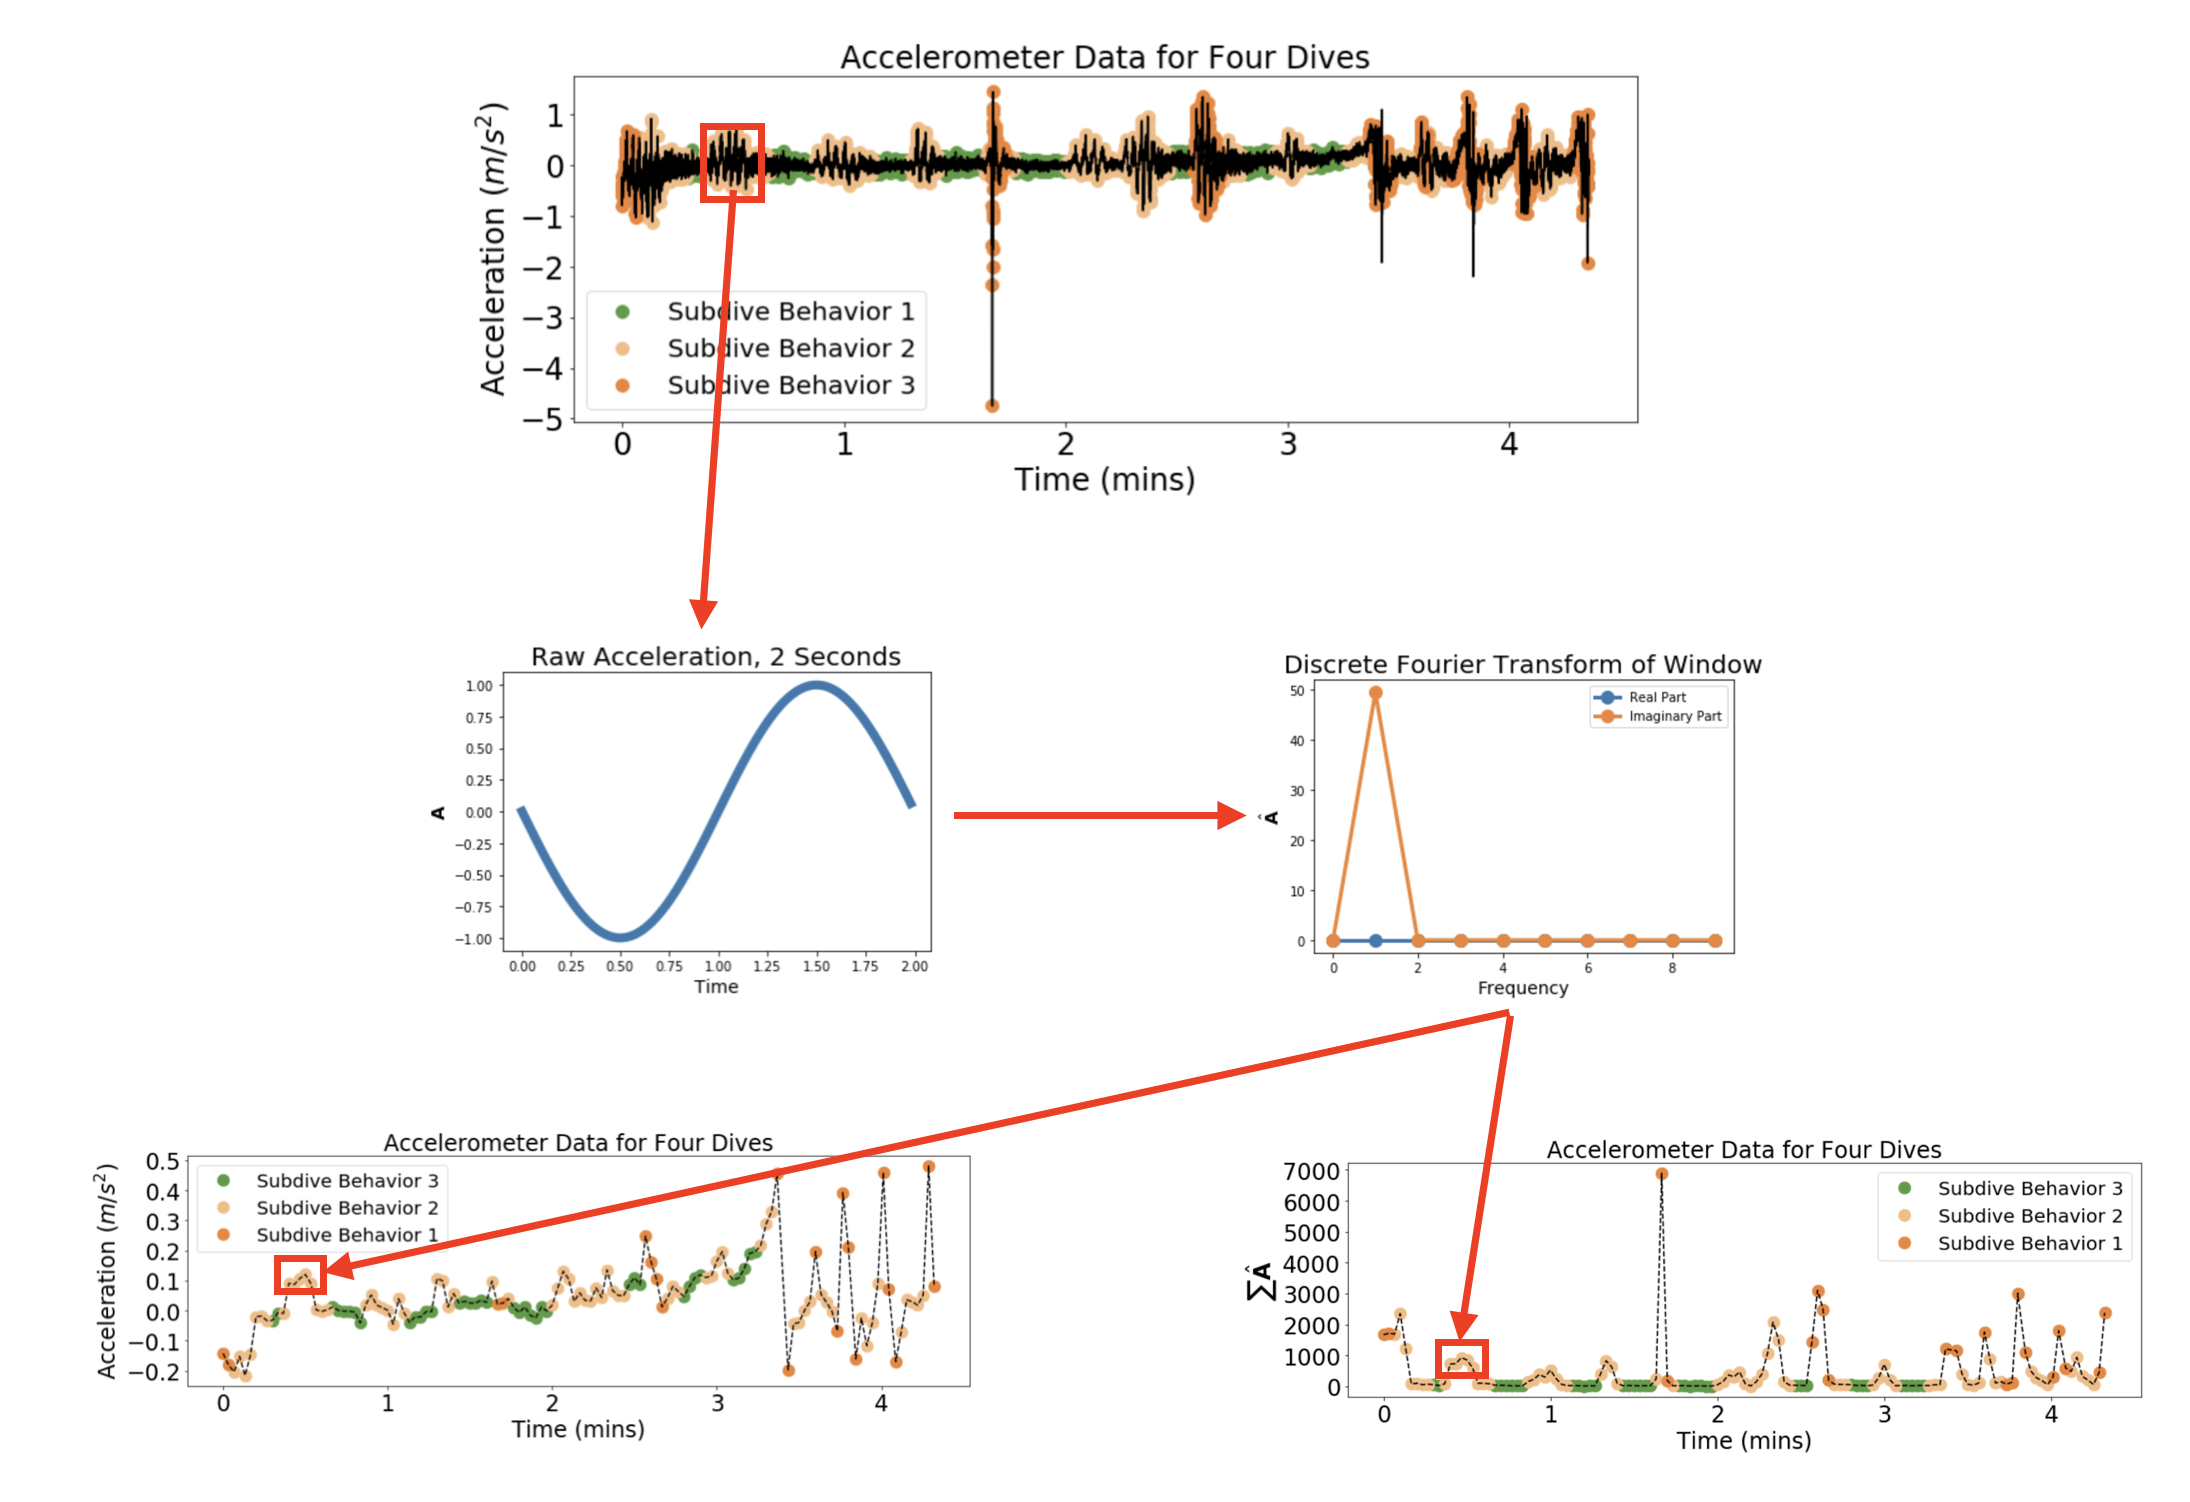
\includegraphics[width=7.5in]{../Plots/fourier_transform.png}
	\caption{Visualization of transforming $Y^*_t$ into $Z^*_t$ using a sliding window and fourier transform.}
	\label{fig:fourier_example}
\end{figure}

Finally, note that it is possible to accommodate for unequal time steps within each window by using the \textbf{non-uniform discrete Fourier transform (NDFT)}. We do not describe the details of this method in this work, but the generalization is straightforward. Refer to Bagchi et al \cite{Bagchi:2001} for details.


\subsection{Model Structure: combining the HHMM and CarHMM}

Hierarchical hidden Markov models can be used to jointly model simultaneous coarse-scale and fine-scale processes taking place simultaneously. However, as mentioned before, the fine-scale process $Y^*$ can often exhibit auto-correlation and intricate structure. Transforming $Y^*_t$ to $Z^*_t$ removes fine-scale periodic behavior, but $Z^*_t$ can still exhibit auto-correlation, especially in the window average, $Z_{t,t^*}^{*(1)}$. Therefore, we replace the fine-scale HMM within the Hierarchical HMM with a CarHMM according to figure (\ref{fig:CarHHMM}).

\begin{figure}[h!]
	\centering
	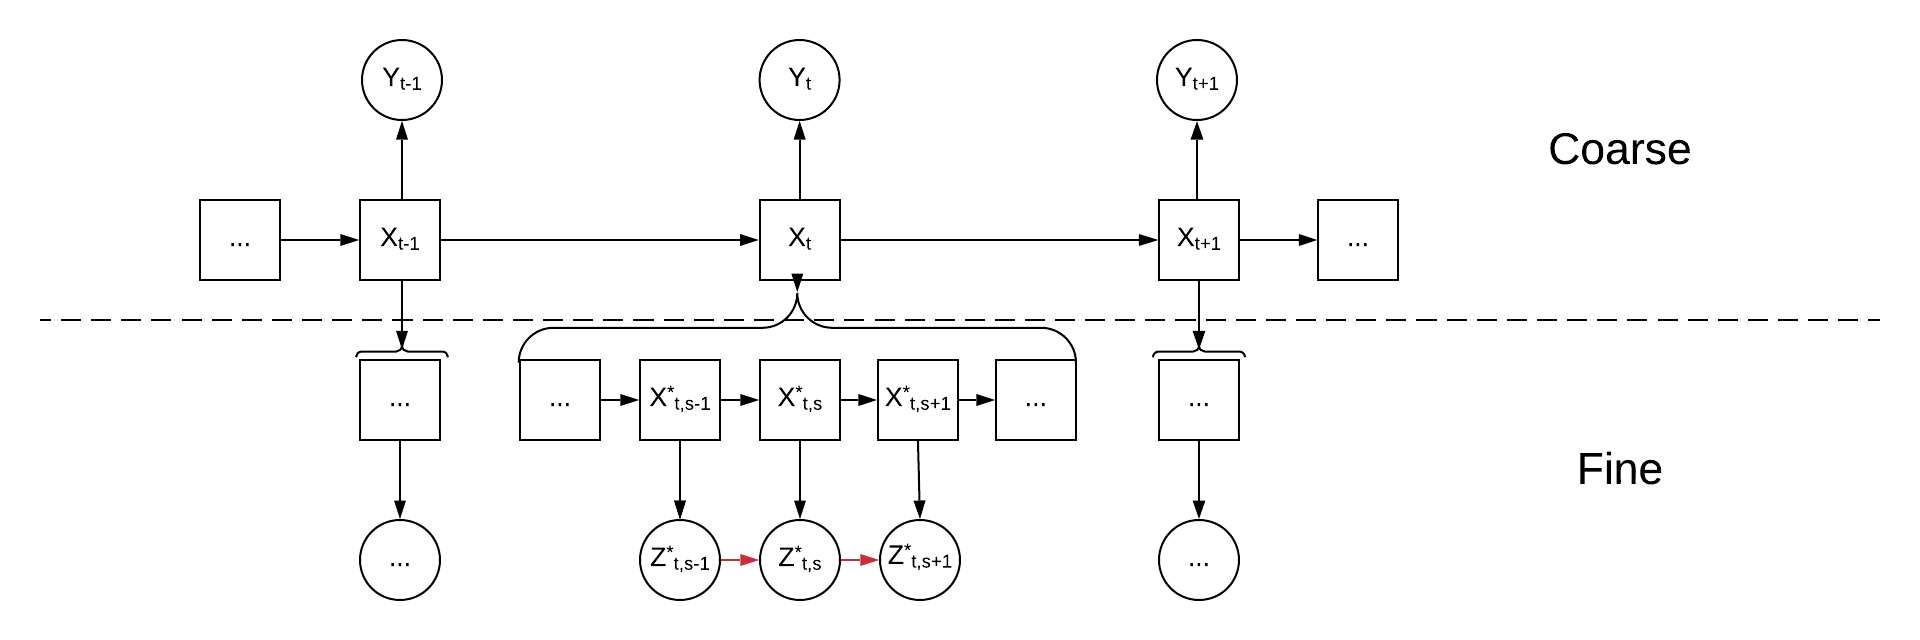
\includegraphics[width=7.5in]{../Plots/CarHHMM.png}
	\caption{Graphical representation of a CarHHMM. The additional arrows representing auto-correlation between observations are shown in red for emphasis.}
	\label{fig:CarHHMM}
\end{figure}

The likelihood of this model is still easy to calculate using the forward algorithm:
%
$$\calL_{\text{CarHHMM}}(y,z^*;\theta,\theta^*,\Gamma,\Gamma^*,\delta,\delta^*) = \delta P(y_1,z_1^*;\theta,\theta^*,\Gamma^*,\delta^*) \prod_{t=2}^T \Gamma P(y_t,z_t^*;\theta,\theta^*,\Gamma^*,\delta^*) \mathbf{1}$$
%
where:
%
\begin{align*}
P(y_t,z_t^*;\theta,\theta^*,\Gamma^*,\delta^*)  = \text{diag}\left[p_{\theta}(y_t|X_t = x_1)\calL_{\text{CarHMM}}\left(z_t^*;\theta^{*(x_1)},\Gamma^{*(x_1)},\delta^{*(x_1)}\right), . . . , \right.\\
\left. p_{\theta}(y_t|x_t = x_N )\calL_{\text{CarHMM}}\left(z_t^*;\theta^{*(x_N)},\Gamma^{*(x_N)},\delta^{*(x_N)}\right) \right]
\end{align*}
%